% --- Configuration ------------------------------------------------------
% add shortcut for github url of this chapter
\def \GITHUB {\GITHUBBASE/03_sound_field_errors_and_their_perceptual_relevance}


% --- Document -----------------------------------------------------------
\chapter{Sound Field Errors and their Perceptual Relevance}
\label{cha:sound_field_errors_and_their_perceptual_relevance}
%
\firstthought{The theory} of sound field synthesis presented so far assumes
continuous secondary source
distributions. With these, any sound field the dimensionality of the
distribution is capable of can be synthesized. The only restriction is that the desired sound
field has to be free of both sources and sinks.

Practical setups cannot meet the assumption which underlies these theoretical
considerations and will introduce errors in the synthesized sound fields.
In this chapter, possible errors will be discussed that are due to
different restrictions of secondary
source setups. In addition, the perceptual relevance of the
different errors will be estimated. For the most relevant errors, perceptual
experiments will be carried out, as further described in Chapter\,\ref{cha:psychoacoustics}.


%--%--%--%--%--%--%--%--%--%--%--%--%--%--%--%--%--%--%--%--%--%--%--%--%--%--%-
\section{Amplitude Errors of \twohalfD Synthesis}
\label{sec:amplitude_errors_of_25d_synthesis}
%
\begin{figure}
    \centering
    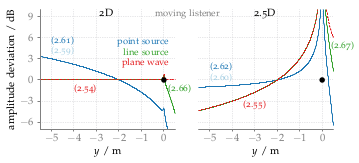
\includegraphics{fig3_01/fig3_01}
    \caption{Amplitudes of sources synthesized via
    \ac{WFS} minus the amplitudes of corresponding real sources
    dependent on the listener's position along
    the $y$-axis. A source is synthesized correctly if its amplitude
    deviation is $0$\,dB. An infinite linear secondary source distribution
    located on the $x$-axis was used, indicated by the black dot.
    A comparison between \twoD and \twohalfD
    synthesis is shown, with the reference point at $\xref = (0,-2,0)$\,m
    for the \twohalfD case. The used driving functions are given within the
    figure.
    Parameters: $f=1$\,kHz.
    \reproduce{\GITHUB/fig3_01}}
    \label{fig:amplitudes}
    \vspace{-0.5cm}
\end{figure}
%
\noindent The possible amplitude decays which can be synthesized depend directly on the
applied secondary sources. Figure\,\ref{fig:amplitudes} shows that a \twoD setup
is not able to synthesize a point source.
The correct amplitude of a point source cannot be synthesized by line
sources as secondary sources, as no stronger amplitude decay than that inherent
to a line source can be achieved.
This solely is a property of the
secondary sources and the dimensionality of the setup and thus independent of
the applied synthesis method.

Due to the mismatch of the secondary source properties and the dimensionality,
deviations of the amplitude are expected in a \twohalfD setup for all synthesized
sources. Figure\,\ref{fig:amplitudes} demonstrates that the deviations for a
synthesized line source or plane wave are the strong\-est ones.
Strong deviations for all sources can be observed especially near the
position of the secondary sources.

%
\begin{figure}
    \centering
    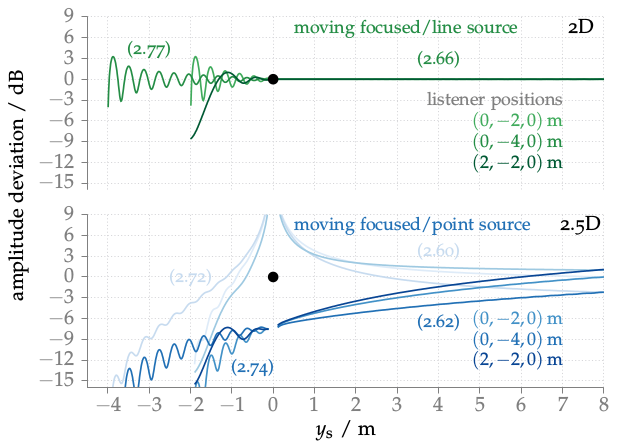
\includegraphics{fig3_02/fig3_02}
    \caption{Amplitudes of a synthesized point/focused source minus the
    amplitudes of corresponding real point source located at $y_\text{s}$
    for three fixed listening positions.
    The secondary source distribution is located on the $x$-axis as
    indicated by the black dot. For positions of the synthesized source with
    negative $y_\text{s}$ values the corresponding focused source models were
    applied. The used driving functions are indicated within the graphs. For the
    \twohalfD case, two different driving functions are shown whereby the dark
    blue one is used as default in this thesis.
    Parameters: $\xref = (0,-2,0)$\,m,
    $f=1$\,kHz.
    \reproduce{\GITHUB/fig3_02}}
    \label{fig:amplitudes_moving_source}
    \vspace{-0.7cm}
\end{figure}
%
\firstthought{In the current} considerations,
only the listener was moved in the audience area. Another case of
amplitude deviations is expected if the listener is at a fixed position and the
synthesized source moves. In the \twohalfD case it should also matter if the listener is
located on the reference point or at another position.
Figure\,\ref{fig:amplitudes_moving_source} shows the case of three fixed
listener positions in a \twoD and a \twohalfD setup. The source is positioned
$8$\,m behind the linear secondary source distribution and moves
towards the listener until it arrives at the listener position.
There are three listener positions, one is at the reference point at $\xref = (0,-2,0)$\,m,
one behind that position and one to the left of it. In the \twoD case, a line source
and the corresponding focused source were synthesized. The line source shows no
amplitude deviations. The focused line source
exhibits deviations in  the form of amplitude ripples. These are not inherent to
the \twoD setup but originate in the finite length of the secondary source
distribution,
which had to be used in the numerical simulation.

In the \twohalfD case, a point source and the corresponding focused source were
synthesized with two different sets of driving functions, as indicated in
Figure\,\ref{fig:amplitudes_moving_source}. The lighter colors represent
the driving functions of a point source and the corresponding focused source
and the darker colors the default driving functions for \ac{WFS} which are
approximations under the assumption of $|\xs-\x0| \gg 1$.
The driving functions without
approximation create sources that have large amplitudes near the secondary source
distribution and have a strong amplitude decay for focused sources.
Völk and Fastl\sidenote[][0cm]{\cite{Volk2012}} investigated this topic and proposed
a correction of the
driving function to create a correct amplitude decay at least at
the reference point -- compare Figure\,5 and 6 in their paper.
With the default driving functions, as shown by the darker color, the sound
field does not exhibit any amplitude
increase near the secondary sources. On the other hand, they lead to a sound
field that shows an overall
decay of the amplitude, which is too strong for an approaching source leading
to a deviation of more than
$-15$\,dB for the simulated geometry.
Away from the reference point, the amplitude has a similar behavior except for
the small offset.


%----%----%----%----%----%----%----%----%----%----%----%----%----%----%----%----
\paragraph{Distance Perception}
%
For \twohalfD synthesis amplitude deviations of a synthesized source can have an influence on the
perceived distance of the synthesized source for \twohalfD synthesis.
In the simulation of a moving source, which is approaching the listener, the
deviations in amplitude could lead to an impression of a
slower approaching source, because the amplitude is not increasing strong
enough, the
closer the source moves to the listener.
In the simulation with a fixed source position and a moving listener, the source
could be perceived as also moving due to its wrong change of amplitude.

Völk has asked listeners to judge the distance of synthesized
point sources in \ac{WFS}.\autocite{Volk2010} The listeners had a fixed position
while the
synthesized source was moved. He applied a driving function with the
same amplitude behavior as~\eqref{eq:D_wfs_ps_25D} -- see
Figure\,\ref{fig:amplitudes_moving_source}. The results for the synthesized
sources are comparable to the results obtained for real sources showing
underestimation of larger distances.\autocite{Zahorik2005}
His results suggest that while having errors in the produced amplitude in
\twohalfD sound field synthesis, the perception of the source is not
modified by these errors.

For nearby sources located closer than $0.5$\,m to the head, changes of the
\ac{ILD} are an important distance cue.\autocite{Brungart1999}
Kerber et al. have shown that \ac{WFS} is not able to recreate the \ac{ILD}
cue for nearby sources.\autocite{Kerber2004}
Otherwise he stated that this might not be so critical if the listener is allowed to
move within the audience area. This was confirmed in an experiment by Müller
et al. in which listeners were supposed to move within the audience area, find the
position of the focused source and grab it.\autocite{Muller2014} The results showed
that listeners succeed with a precision of around $15$\,cm.

Besides the distance cues discussed so far, the direct-to-reverberant energy
ratio plays a large role for distance perception inside of
rooms.\autocite{Bronkhorst1999}
Results from the literature indicate that due to the reflections of the signals
from the secondary sources, the direct-to-reverberant energy ratio will be
different for \ac{WFS} and possibly influences the perception.\autocite{Volk2010a}

\newthought{The majority of} experiments of distance perception in \ac{SFS}
concentrated on a
single position of the listener. One of the goals of this thesis is to investigate the
perception in an area as large as possible. This suggests to use the method of
binaural synthesis -- presented in the next chapter -- to investigate the
perception of distance. In a critical manner the perceived distance is highly
influenced by the binaural simulation.\sidenote[][-0.8cm]{\cite{Hartmann1996}}
As a consequence, distance perception is not considered in this thesis.


%--%--%--%--%--%--%--%--%--%--%--%--%--%--%--%--%--%--%--%--%--%--%--%--%--%--%-
\section[Diffraction and Truncation]{Diffraction and Truncation of Secondary Source Distributions}
\label{sec:diffraction_and_truncation_of_secondary_source_distributions}
%
\begin{figure*}
    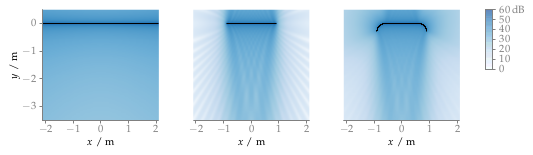
\includegraphics{fig3_03/fig3_03}
    \caption{Sound pressure in decibel of a plane wave synthesized with
    \twohalfD \ac{WFS}~\protect\eqref{eq:D_wfs_pw_25D}.
    The result of an infinite linear secondary source distribution is
    compared with two truncated ones. Parameters: $\n_k = (0,-1,0)$, $\xref =
    (0,-2,0)$\,m $f = 3$\,kHz.
    \reproduce{\GITHUB/fig3_03}}
    \label{fig:sound_field_truncation}
\end{figure*}
%
\noindent The solutions for a linear secondary source distribution assume an infinite
length of the distribution, which typically is violated in a real-life
setup, where lengths of around $3$\,m are common. This provok\-es errors in the
synthesized sound field that can be described by diffraction theory. The
linear source distribution can be thought of as a slit where a wave field
coming from the other side has to go through. The slit can be modelled as
a rectangle window, the corresponding diffraction pattern is that of a sinc
function as shown in Ahrens.\autocite[][(3.87)]{Ahrens2012}
Figure\,\ref{fig:sound_field_truncation} displays the sound pressure level
of a synthesized plane wave
going into the direction $(0,-1,0)$ for an infinite linear secondary source
distribution and a distribution with a length of $1.8$\,m. The array's form
influences the diffraction pattern as can be seen for the
secondary source distribution to the right. In this case, it is covering
$1.8$\,m like in the case depicted in the middle,
but the edges of the array are bend towards the listening area. In this way the diffraction
pattern is pronounced to a lower degree than before, emphasizing that the edges
have a large impact on the diffraction.

This can be further highlighted with an
equivalent description of the diffraction by so called edge waves.
Consider that the length of the secondary source distribution is large
compared to the wave
length of the sound, but small compared to the distance between the
source position $\x_0$ and the receiver position $\x$. In addition,
the incidence angle of the sound is approximately
vertical to the secondary sources. In this case the problem can be approximated by
\emph{Kirchhoff's diffraction theory}.\autocite[][Sect.\,8.3.2.]{Born1999}
Here, the
diffraction can be explained in an equivalent manner
by a super-position of the incident
sound field and two spherical waves originating from the edges of the array --
this is well summarized in Born and Wolf.\autocite[][Sect.\,8.9]{Born1999}
\FloatBarrier% fix maximum number of allowed floats
The same was found for \ac{WFS} by Verheijen\autocite{Verheijen1997} and
by Start\autocite{Start1997} -- where the diffraction for \ac{WFS} is
treated in more mathematical detail.
They introduced a so called tapering window to
attenuate the edge waves by reducing the amplitude of the secondary sources at the
edges with cosine windows. For investigating the influence of the window
function, Ahrens' approach to transform the problem into the $k_x$-domain can be
useful.\autocite[][Sect.\,3.7.4]{Ahrens2012}

The edge waves and their reduction by the tapering window are shown in
Figure\,\ref{fig:tapering}. There, three cosine shaped pulses are synthesized as
plane waves traveling downwards. Looking at the amplitudes for the line at $x
= 0$\,m parallel to the $y$-axis the influence of the tapering can be estimated.
In the left figure the level of the edge wave is approximately $20$\,dB lower than
that of the
desired wave front. In the right figure, including the tapering window, the edge
wave is attenuated by $10$\,dB and thereby is $30$\,dB below the desired wave
front.
%
\begin{figure}
    \centering
    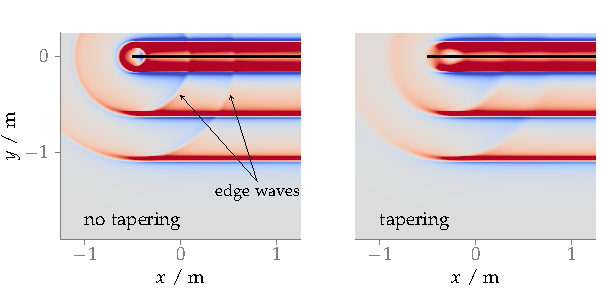
\includegraphics{fig3_04/fig3_04}
    \caption{Sound pressure of three cosine shaped broad-band pulses
    synthesized as plane waves with \ac{WFS}~\protect\eqref{eq:d_wfs_pw_25D}.
    Additional edge waves are visible due to diffraction.
    By applying a tapering window to the last $30$\,cm of the secondary source
    distribution the edge waves could be damped, as is shown in the
    right graph.
    Parameters: $\xs =(0,-1,0)$, $\xref = (4.5,-2,0)$\,m, $t = 4.6$\,ms.
    \reproduce{\GITHUB/fig3_04}
    }
    \label{fig:tapering}
\end{figure}
%

Diffraction occurs also for non-smooth array contours that include a corner. In
this case the level of an additional diffraction wave is negligible, as shown
in Verheijen\autocite[][Fig.\,2.22]{Verheijen1997} and
Ahrens\autocite[][Fig.\,3.26 and 3.27]{Ahrens2012}.

\newthought{Another influence} of the truncation is of interest only for focused
sources.
Size and shape of the secondary source distribution have an influence on
the extent of the focal point. The extent of the focal point should be given by
the first two minima's distance in the diffraction pattern.
With an infinite linear secondary source distribution the size of the 
focal point is $\lambda$.\sidenote[][-2cm]{\cite[][formula on p.\,26 with $n=1$
and $\omega=\nicefrac{\pi}{2}$; the result is $\nicefrac{\lambda}{2}$
for a microscope, because the resolution is defined as the distance between the
first maximum and minimum of the diffraction pattern.]{Abbe1880}}
However, for a truncated array the focal point can get larger.
Under the assumption of
\emph{Fraunhofer diffraction},\autocite[][Sect.\,8.3, (34). Diffraction
for a focal point is equivalent to diffraction for plane waves coming from
infinity and focus them by a lens -- compare Figure\,8.6.
For plane waves from infinity eq.\,34 is automatically fullfilled.]{Born1999}
the size can be
calculated as the distance between the first zeros of the diffraction pattern.
The first zeros result for a path difference of $\lambda$ of the two waves
originating from the slit's edges.
Figure\,\ref{fig:diffraction_slit} shows the setting for a linear secondary
source distribution located on the $x$-axis. The angle
$\alpha$ is obviously given by $\sin\alpha =
\nicefrac{\lambda}{L}$, and the focal point size for a linear secondary source
distribution is then 
given as\autocite[][(13)]{Wierstorf2013a}
%
\begin{marginfigure}
    \centering
    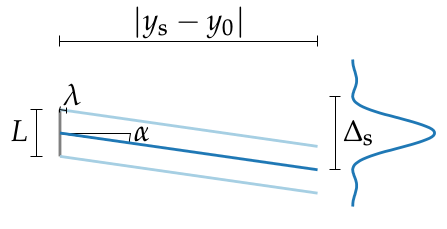
\includegraphics{fig3_05/fig3_05}
    \caption{Size of the focus point $\Delta_\text{s}$ as given by Fraunhofer
    diffraction.
    \reproduce{\GITHUB/fig3_05}}
    \label{fig:diffraction_slit}
\end{marginfigure}
%
\begin{equation}
    \Delta_\text{s} =
    \left[ 2|y_\text{s}-y_0| \tan\left(\sin^{-1} \frac{\lambda}{L}
    \right), \lambda \right]_\text{max} \qc
    \label{eq:focus_size}
\end{equation}
where $L$ is the length of the
truncated secondary source distribution, and $\lambda = \nicefrac{c}{f}$ the wave
length.
%
\begin{figure*}[t]
    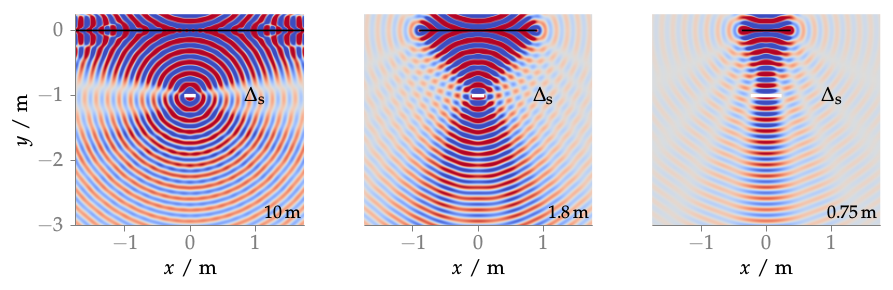
\includegraphics{fig3_06/fig3_06}
    \caption{Sound pressure of a focused source synthesized with
    \twohalfD \ac{WFS}~\protect\eqref{eq:D_wfs_fs_25D}.
    Three different linear secondary source distributions were
    applied, ranging from $10$\,m to $0.75$\,m. In white the size of the focal
    point as given by $\Delta_{\text{s},\,\text{linear}}$ is
    indicated. Parameters: $\xs = (0,-1,0)$\,m, $\xref = (0,-2,0)$\,m, $f =
    2000$\,Hz.
    \reproduce{\GITHUB/fig3_06}
    }
    \label{fig:focal_point_size}
\end{figure*}
%
In Figure\,\ref{fig:focal_point_size} the size of the focal point is shown
for different lengths of a linear secondary source distribution and a wave
length of $\lambda = 0.172$\,m. The size of the focal point calculated
with~\eqref{eq:focus_size} is
$0.47$\,m, $0.19$\,m, $0.17$\,m going from the smallest distribution to the
largest one -- from left to right. The real sizes that can be examined by analyzing the
amplitude distribution in the focal plane of the simulated sound field
are $0.50$\,m, $0.24$\,m, $0.14$\,m.
The result shows that a smaller secondary source distribution leads to a wider
focal point. In addition, the focal point will become even larger for lower
frequencies, as can directly be seen from~\eqref{eq:focus_size}.
Note that the focal point size can also be calculated with (24) from Lucas
and Muir\sidenote[][1cm]{\cite{Muir1982}} which generates similar results.

For a circular secondary source distribution in most cases the focal point size
can be approximated by $\lambda$. The concave shape of the distribution allows
a better focussing of the sound field.

The right graph of Figure\,\ref{fig:focal_point_size} highlights another phenomenon for small
secondary source distributions and low frequencies: the focal point
shifts towards the secondary sources. This is discussed in detail by
Oldfield,\autocite[][Sect.\,4.9]{Oldfield2013} who also proposes a method to
correct the shift for the synthesis of focused sources.


%----%----%----%----%----%----%----%----%----%----%----%----%----%----%----%----
\paragraph{Perception}
%
After discussing the various physical influences of truncating the secondary
source distribution, in the following a short summary of its potential influence on the
perception is presented.

The strongest influence of truncating the secondary source distribution is on the
size of the listening area which becomes smaller dependent on the exact size of
the distribution and the synthesized source -- compare
Figure\,\ref{fig:sound_field_truncation} and \ref{fig:focal_point_size}.
If the listener is placed at the
border
of the listening area, the truncation could influence the localization of a
synthesized source. Having the center of the head exactly at the border will
lead to one ear in the listening area and one ear being out of it, provoking a
possibly large \ac{ILD} between the two ears. Depending on the amount of level
difference and uncertainty in the other localization cues, the \ac{ILD} could
dominate the localization perception. The perceived source direction then is
very likely to be in another direction than the one desired for the synthesized source.
For a mono-frequent source with low frequency a wrong \ac{ILD} could also be
possible within the listening area because of the maxima and minima of the
diffraction pattern.

The diffraction due to the truncation by the secondary source distribution can
be described in an equivalent way by edge waves starting at the edges of the
distribution. For a listener at a certain position within the
listening area this means that she will at first hear the desired sound, and shortly afterwards
one or two reflections of the same sound coming from the edges of the
distribution. If the distribution is not larger than $4$\,m, this probably does not have
any influence on the localization, due to the precedence
effect\autocite[A good summary is provided in][]{Litovsky1999} which
ensures a domination of the perceived direction by the first arriving sound.
However, the additional edge waves will add some sort of coloration to the perceived
sound.
The edge waves can easily be damped by applying a tapering window.
%Moreover,
%the additional wave fronts due to the discretization of the
%secondary source distribution will have a larger influence.
As this effect can easily be avoided, no perceptual experiments were carried out to
investigate the influence of the edge waves.

Beside the fact of wrong \ac{ILD} cues at the margins of the listening area the
truncation can have further influence on the localization for focused
sources. As shown in Figure\,\ref{fig:focal_point_size} the size of the focal
point depends on the size of the secondary source distribution. A larger focal
point will most probably widen the perceived source width. If size of the focal
point further increases, it may further be shifting the perceived position of the
focused source towards the secondary source distribution.

To investigate the influence of the truncation on the localization of
focused sources, a localization experiment for focused sources synthesized with
different secondary source distributions will be presented in
Chapter.\,\ref{cha:psychoacoustics}.


%--%--%--%--%--%--%--%--%--%--%--%--%--%--%--%--%--%--%--%--%--%--%--%--%--%--%-
\section[Spatial Aliasing and Discretization]{Spatial Aliasing and Discrete Secondary Source Distributions}
\label{sec:spatial_aliasing_and_discrete_secondary_source_distributions}

%
\begin{figure}
    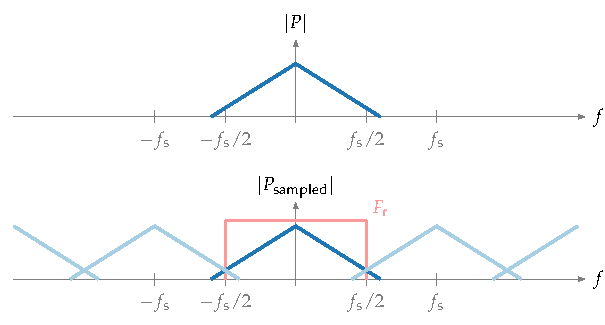
\includegraphics{fig3_07/fig3_07}
    \caption{Magnitude of a continuous signal $P$ and the same signal
    sampled with a sampling frequency of $f_\text{s}$. The light blue lines
    indicate components occurring due to the sampling process. $F_\text{r}$
    describes an ideal reconstruction filter for the sampled signal.
    \reproduce{\GITHUB/fig3_07}}
    \label{fig:sampling}
\end{figure}
%
\noindent Up to now, only continuous secondary source distributions have been
considered, that can hardly be built up in practice. Normally, an array of
loudspeakers is applied which corresponds to a sampling of the secondary source
distribution in space. This leads to different impacts on the synthesized sound
field.

For a better understanding of the phenomenon a comparison of the temporal
sampling of a signal is of interest. Consider a signal $p(t)$ and its Fourier
transform $P(\omega)$ with $\omega = 2\pi f$. The signal will be sampled with a
sampling frequency of $f_\text{s}$ which means that only its values at multiplies of
$\Delta t = \nicefrac{1}{f_\text{s}}$ are considered. Figure\,\ref{fig:sampling}
illustrates the consequences of the sampling process. The sampled signal
$P_\text{sampled}$ now includes spectral repetitions of the original signal at
each multiple
of $f_\text{s}$. If the original signal should be recreated from the sampled
one, a reconstruction filter $F_\text{r}$ as indicated by the red line in
Figure\,\ref{fig:sampling} has to be applied to the signal.
If the sampled signal contains frequencies larger than
$\nicefrac{f_\text{s}}{2}$, they will overlap and interfere with the base band
and the signal will be corrupted by \emph{aliasing}.
Thus, the frequency $\nicefrac{f_\text{s}}{2}$
can be defined as the aliasing frequency $f_\text{al}$ depending on the
distance of the sample points as
%
\begin{equation}
    f_\text{al} = \frac{1}{2\Delta t} \qp
    \label{eq:fal_time}
\end{equation}
%

Now, the same problem with a driving function $D(x_0)$ and a one-dimensional
secondary source distribution is considered. In this case the secondary source
distribution will be sampled at multiples of $\Delta x_0 =
\nicefrac{2\pi}{k_x}$ and spectral repetitions
of the sampled driving function will occur in the $k_x$ domain. Due to the
dispersion relation $k^2 = (\nicefrac{\omega}{c})^2$ a spatial
aliasing frequency here can be specified as
%
\begin{equation}
    f_\text{al} = \frac{c}{2\Delta x_0} \qc
    \label{eq:fal}
\end{equation}
%
where $c$ is the speed of sound.

The secondary sources themselves can be considered as the reconstruction filter in this case.
Because of the dispersion relation only their propagating parts are band-limited in
the spatial domain up to a given frequency $f$. Both spatial
aliasing due to interference of repetitions with the base band and
reconstruction errors due to the suboptimal suppression of spatial repetitions
can occur in the sound field.
For some examinations it could be useful to distinguish between these two
cases,\autocite[][Chap.\,4 deals with the discretization of
different secondary source distribution in great detail.]{Ahrens2012} but for the
perceptually relevant aspects discussed in this thesis they will be subsumed
jointly under the term spatial aliasing. Hence, the spatial aliasing frequency
as used here covers both cases.

\newthought{In three dimensions} with $\k = (k_x,k_y,k_z)$ and $\x_0 = (x_0,y_0,z_0)$ the
aliasing frequency specified by~\eqref{eq:fal} is only a lower boundary. Now
the amount of spatial aliasing will become dependent on the
position and on the type and position of the synthesized source. In the
following, the dependency
on the position of the listener is explained by an example. Consider
a linear secondary source distribution and a listener facing the
distribution. Assuming the listener is as close as
possible to the secondary source distribution standing between two individual
secondary sources. In this case, the sound could reach her
from directions ranging from $-90\degree$ to $90\degree$ relative to her head
orientation. If the
listener is as far away from the distribution as possible the sound reaching her
ears from the same two individual secondary sources
arrives from the same direction of $0\degree$. That means with increasing
distance of the listener from the secondary source distribution
less spatial frequencies are needed to represent the signal at the listener
position.

%
\begin{figure*}[t]
    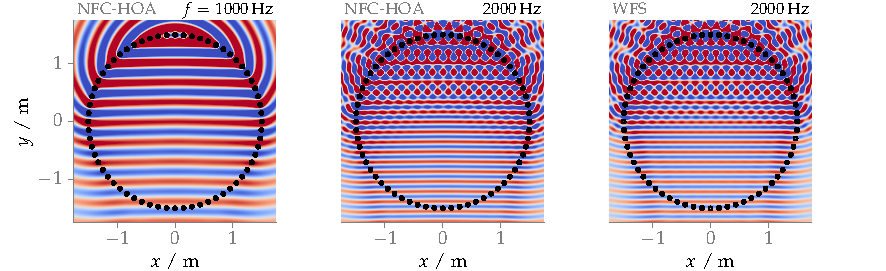
\includegraphics{fig3_08/fig3_08}
    \caption{Sound pressure of a plane wave synthesized by
    \ac{NFC-HOA}~\protect\eqref{eq:D_nfchoa_pw_25D} and
    \ac{WFS}~\protect\eqref{eq:D_wfs_pw_25D} for different frequencies.
    For \ac{WFS} the open circles indicate inactive secondary sources.
    Parameters: $\xs = (0,-1,0)$, $\xref = (0,0,0)$\,m, 64 secondary sources. 
    \reproduce{\GITHUB/fig3_08}}
    \label{fig:aliasing}
\end{figure*}
%
Figure\,\ref{fig:aliasing} shows aliasing phenomena for \ac{NFC-HOA} and
\ac{WFS} for a
circular secondary source distribution. The secondary source distribution
is sampled at $64$
discrete points leading to a lower boundary of the aliasing frequency of
$1165$\,Hz. This can be observed in the figure as well. For a frequency of
$1000$\,Hz the synthesized sound field will be free from aliasing, but for a
frequency of $2000$\,Hz aliasing occurs at points near the secondary source
distribution. Furthermore, it can be observed that the pattern of aliasing is nearly
identical in the case of \ac{NFC-HOA} and \ac{WFS}. 

As mentioned before the amount of spatial aliasing depends on the type
and position of the synthesized source. This is due to the fact that for most
of the source types and positions the sampling of the
secondary source distribution is irregular in space. In this case
nonuniform sampling theory has to be applied to determine the right spatial aliasing
frequency. There are suggestions how to calculate it for the synthesis of point
sources\autocite{Corteel2006} and for focused sources\autocite{Oldfield2013},
but no general solution has been presented so far, and is out of scope for
this thesis.
If the aliasing frequency is needed for a
defined configuration, it will be
determined by numerical simulation of the situation and inspection of the
spectrum -- compare Figure\,\ref{fig:freq_response}.
However, in most cases it will be sufficient to use~\eqref{eq:fal} as an approximation of
the aliasing frequency. Only for a synthesized focused source special
considerations are necessary.

%
\begin{figure*}[b]
    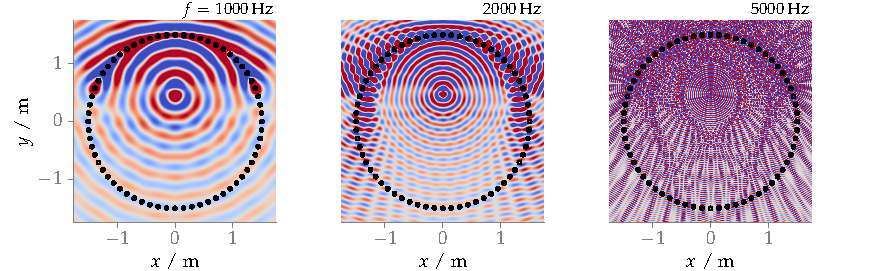
\includegraphics{fig3_09/fig3_09}
    \caption[][-0.9cm]{Sound pressure of a focused source
    synthesized by
    \ac{WFS}~\protect\eqref{eq:D_wfs_fs_25D} for different frequencies. Parameters:
    $\xs = (0,0.5,0)$, $\xref = (0,0,0)$\,m, 64 secondary sources.
    \reproduce{\GITHUB/fig3_09}}
    \label{fig:aliasing_fs}
\end{figure*}
%
Figure\,\ref{fig:aliasing_fs} shows the
amplitude of the sound field of a focused source placed at $(0,0.5,0)$\,m
synthesized with \twohalfD \ac{WFS}. It indicates that for high frequencies
there always is a circular region around the focal point where no aliasing
occurs. This property of a correct synthesis in a small region with the help of
a focused source has already been used in different applications where a
small but aliasing-free region should be
synthesized.\autocite[E.g.][]{Spors2010b}
For a linear secondary source distribution located on the $x$-axis
the radius $r_\text{al}$ of the aliasing-free zone was empirically found
in Wierstorf et al\autocite[][(12)]{Wierstorf2013b} as
%
\begin{equation}
    r_\text{al} = \frac{y_\text{s}c}{f\Delta x_0} \qp
\end{equation}

\newthought{The idea} of a spatially limited but aliasing free region can be applied in
\ac{NFC-HOA} in a more direct way by limiting the spatial bandwidth of the driving
function. The lower orders of the Bessel functions contribute to a higher degree to the sound
field in the center of the secondary source distribution, whereas higher orders
contribute more to positions at distances far from the
center.\autocite[][Sect.\,2.2.2]{Ahrens2012}
Hence, a correctly synthesized region in the center of the
secondary source distribution for a limited order is expected.
In order to avoid spatial aliasing the maximum
order $M$ should be smaller or equal to $\nicefrac{\pi}{x_0}$. For a circular
secondary source distribution the maximum order without spatial aliasing is then
given as
\urlnote{nfchoa\_order.m}{\SFS/SFS_general/nfchoa_order.m}
%
\begin{equation}
    M \le
    \begin{cases}
        \nicefrac{(N_\text{s}-1)}{2} & \text{for even } N_\text{s} \\
        \nicefrac{N_\text{s}}{2} & \text{for odd } N_\text{s} \qc
    \end{cases}
    \label{eq:nfchoa_order}
\end{equation}
%
where $N_\text{s}$ is the number of secondary sources.

\begin{figure}
    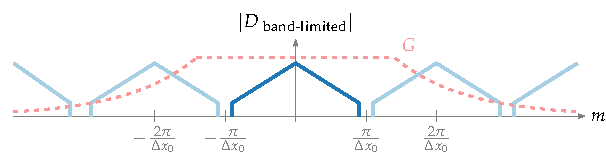
\includegraphics{fig3_10/fig3_10}
    \caption{Magnitude of a mono-frequent, spatial band-limited \ac{NFC-HOA}
    driving function.
    The light blue lines
    indicate components occurring due to the sampling process. $G$ describes the
    reconstruction filter.
    \reproduce{\GITHUB/fig3_10}}
    \label{fig:sampling_band_limited}
\end{figure}
%
\begin{figure*}[b]
    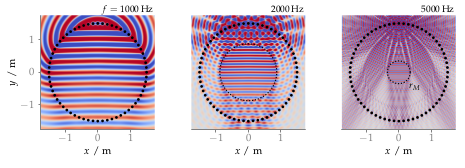
\includegraphics{fig3_11/fig3_11}
    \caption[][-0.9cm]{Sound pressure of a plane wave synthesized by
    \ac{NFC-HOA}~\protect\eqref{eq:D_nfchoa_pw_25D} for different frequencies.
    The maximum order $M$ was set
    to be $32$ after~\protect\eqref{eq:nfchoa_order}. The region of correct synthesis is
    given by $r_M = \nicefrac{Mc}{\omega}$ as indicated by the dotted line.
    Parameters: $\xs = (0,-1,0)$, $\xref = (0,0,0)$\,m, 64
    secondary sources.
    \reproduce{\GITHUB/fig3_11}}
    \label{fig:nfchoa_aliasing}
\end{figure*}
%
Figure\,\ref{fig:sampling_band_limited} shows the effect of band-limiting.
Here, the spectral repetitions of the driving
function no longer interfere with each other. On the other hand, the reconstruction
filter -- the Green's function $G$ -- 
in general is not band-limited. Above a certain frequency spectral repetitions
will be part of the synthesized sound field. Figure\,\ref{fig:nfchoa_aliasing}
presents the amplitude distribution of the sound field for a plane wave with
direction $(0,-1,0)$ synthesized by
\twohalfD band-limited \ac{NFC-HOA} using a circular secondary source distribution with
$64$ sources and a radius of $1.5$\,m. For a frequency of $1$\,kHz the sound field
is synthesized without errors, while for $2$\,kHz and $5$\,kHz only a region in the
center of the distribution is synthesized correctly. The size of that region is
given as\autocite[Compare (9.1.31) and Fig.\,9.5 of][]{Gumerov2004}
%
\begin{equation}
    r_M = \frac{Mc}{\omega} \qp
    \label{eq:rM}
\end{equation}
%
As a result of reconstruction errors outside of the $r_M$ region, spatial aliasing occurs.
In contrast to the spatial aliasing in the synthesized sound field for a
full-band synthesis as shown in Figure\,\ref{fig:aliasing} the reconstruction errors
introduce amplitude fluctuations outside of the $r_M$ region.

\newthought{The influence} of the spatial aliasing on the signals at a given
listener position can further be analyzed by the corresponding temporal-frequency
spectrum at a given position.
Figure\,\ref{fig:freq_response} shows the magnitude of the spectrum at
three different listener positions. Synthesizing a plane wave
with a circular secondary source distribution with a radius of $1.5$\,m in all
cases, a continuous secondary source distribution or a sampled one with 64 sources was
driven by \ac{WFS}, \ac{NFC-HOA} or band-limited \ac{NFC-HOA}. For the
continuous distribution for all listener positions the spectrum is flat
for \ac{NFC-HOA} and \ac{WFS}. Only for frequencies below $400$\,Hz some slight
deviations are visible for \ac{WFS}. That is not surprising as \ac{WFS} is a
high-frequency approximation of \ac{NFC-HOA}.
%
\begin{figure*}[t]
    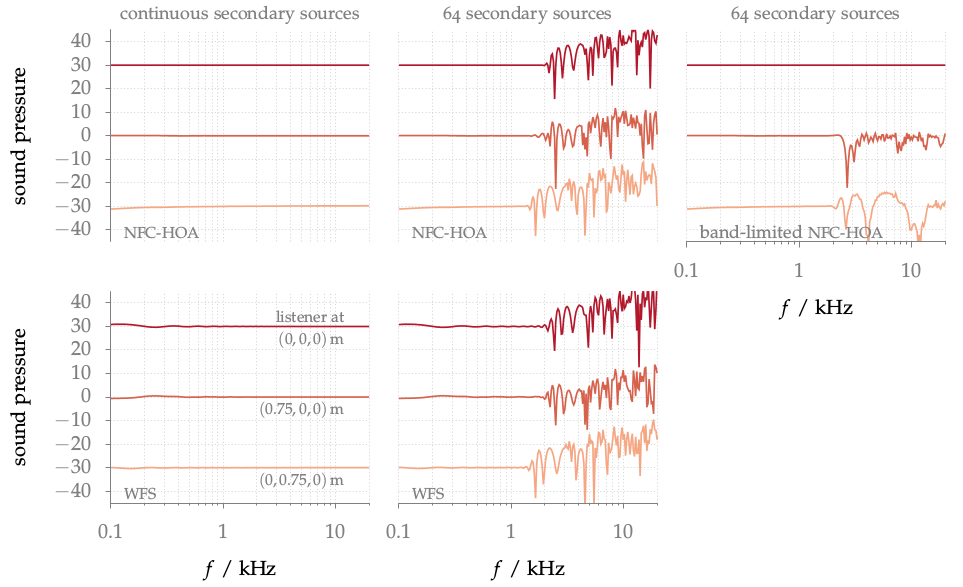
\includegraphics{fig3_12/fig3_12}
    \caption[][-3.5cm]{Sound pressure in decibel of a plane wave synthesized by
    \ac{NFC-HOA}~\protect\eqref{eq:D_nfchoa_pw_25D} and
    \ac{WFS}~\protect\eqref{eq:D_wfs_pw_25D}. Mono-frequent simulations were
    done for all frequencies at three different listening positions. A fixed
    offset was added to the amplitudes for two of the positions for better
    visualization.
    Parameters: $\xs = (0,-1,0)$, $\xref = (0,0,0)$\,m, circular secondary
    source distribution with a diameter of $3$\,m.
    \reproduce{\GITHUB/fig3_12}}
    \label{fig:freq_response}
\end{figure*}
%

The sampling with only 64 secondary sources introduces aliasing artifacts at all listener
positions. The figure indicates that these artifacts appear only above a given
aliasing frequency and are position dependent. The lower limit of the aliasing
frequency can be calculated with~\eqref{eq:fal} as $1165$\,Hz
which is exceeded by the aliasing frequency observed in
Figure\,\ref{fig:freq_response}
at all three of the investigated listener positions. The
aliasing not only introduces fluctuations to the magnitude spectrum but
in addition adds energy to the spectrum with a slope of $3$\,dB per octave.
While
this slope is identical to the slope of the pre-equalization
filter~\eqref{eq:d_wfs_pw_25D} it is common practice in \ac{WFS} to apply this
filter only up to the aliasing frequency. The experiments presented in this
thesis also use this practice.

In addition to \ac{NFC-HOA}, the sampled secondary sources were also driven by
band-limited \ac{NFC-HOA}. As expected, this results in no aliasing for the
central listening position. Outside of the center the problem remains, although
the pattern of deviations in the spectrum differs and the $3$\,dB slope is
missing completely.

The spatial aliasing artifacts are not only visible in the spectrum of the
synthesized sound field, but also manifest themselves in the temporal signals at
a fixed listener position.


%----%----%----%----%----%----%----%----%----%----%----%----%----%----%----%----
\newthought{The temporal signals} of the sound field provide additional insights
on the properties of the spatial aliasing artifacts.
%
\begin{figure*}[tb]
    \vspace{-0.5cm}
    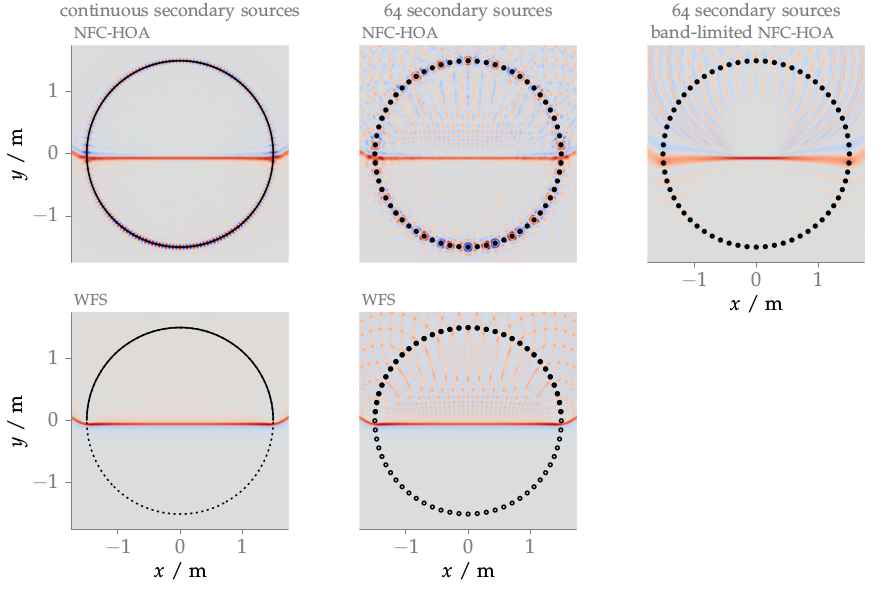
\includegraphics{fig3_13/fig3_13}
    \caption[][-3cm]{Sound pressure of a cosine shaped impulse synthesized as a
    plane wave by \ac{NFC-HOA}~\protect\eqref{eq:D_nfchoa_pw_25D} and
    \ac{WFS}~\protect\eqref{eq:d_wfs_pw_25D}. Parameters:
    $\xs = (0,-1,0)$, $\xref = (0,0,0)$, $t = 4.6$\,ms, 64 secondary sources for
    the sampled distributions.
    \reproduce{\GITHUB/fig3_13}}
    \label{fig:sound_field_imp}
\end{figure*}
%
A broad band pulse is synthesized and after some time $t$ the sound
field is frozen and plotted. Figure\,\ref{fig:sound_field_imp} demonstrates the
synthesized sound field of a ten samples long, Hann-window shaped pulse after $t = 4.6$\,ms for
different setups. The top row represents \twohalfD \ac{NFC-HOA} for a continuous
secondary source distribution and a discrete one with $64$ sources. For the
latter in addition the result for \ac{NFC-HOA} is shown in the graph to the
right. The bottom row shows the same sound fields synthesized with \twohalfD
\ac{WFS}.
Band-limited \ac{WFS} has not been investigated so far and will be omitted in this
thesis.

The results for the full-band cases are similar
between \ac{NFC-HOA} and \ac{WFS}. For a continuous secondary source distribution the
pulse is synthesized without errors.
For discrete secondary sources additional wave fronts
are visible which arrive after the desired pulse and have a similar pattern for
both methods.
The large magnitudes near the secondary sources in the case of \ac{NFC-HOA} are
most likely due to numerical problems. These are inherent to the calculation of
higher order components,\footnote{In order to calculate orders higher than 85 at
all the \href{http://www.advanpix.com/}{\color{link}Multiprecision Computing
Toolbox}
for
Matlab was applied for finding the zeros of the Bessel function -- compare
\url{sphbesselh\_zeros.m}{\SFS/SFS\_general/sphbesselh\_zeros.m}}
which should be most prominent near the
secondary sources.
For the band-limited \ac{NFC-HOA} case the pulse is synthesized
correctly in the center of the distribution, but again has additional signal
components outside of the center.

\begin{figure*}[tb]
    \vspace{-0.5cm}
    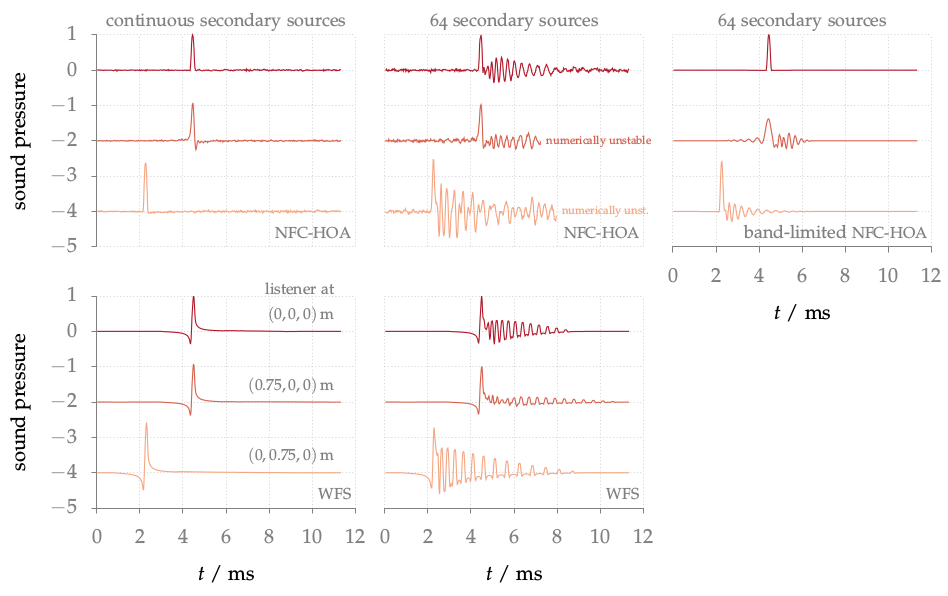
\includegraphics{fig3_14/fig3_14}
    \caption[][-3cm]{Sound pressure of cosine shaped impulse synthesized as a
    plane wave by \ac{NFC-HOA}~\protect\eqref{eq:D_nfchoa_pw_25D} and
    \ac{WFS}~\protect\eqref{eq:d_wfs_pw_25D} at three different listening
    positions. A fixed offset was added to the sound pressure at two listening
    positions for a better visualization.
    Parameters: $\xs = (0,-1,0)$, $\xref=(0,0,0)$, circular secondary source
    distribution with a diameter of $3$\,m.
    \reproduce{\GITHUB/fig3_14}}
    \label{fig:sound_field_imp_fixed}
\end{figure*}
%
A further investigation of the exact temporal pattern of the wave
fronts at three different listener positions is presented in
Figure\,\ref{fig:sound_field_imp_fixed}. Here, the following positions were
chosen: one at the center
$(0,0,0)$\,m, one in the frontal part of the audience area $(0,0.75,0)$\,m, and
one in the right part of the audience area $(0.75,0,0)$\,m. The
figure reveals only few errors in the temporal pattern for the synthesis of
the plane wave with a continuous secondary source distribution.
Additionally in this case, for all three positions the Hann-window shaped pulse is synthesized
correctly. In the case of \ac{NFC-HOA} the amplitude shows more noise than
for \ac{WFS},
again likely due to numerical limitations in the calculation of the \ac{NFC-HOA}
driving functions.
\ac{WFS} constitutes a high-frequency approximation of the exact \ac{SFS}
solution, which explains the slight undershoots at the beginning of the impulse
for \ac{WFS}.

For a sampled secondary source distribution, errors are visible in all cases. Now
additional positive and negative pulses are evident after the first one. Again
the pattern is very similar for \ac{WFS} and \ac{NFC-HOA}. For the latter, 
numerical instabilities could not be solved for parts of the signal.
Hence, parts of it are omitted in the figure.
The time window during which  the additional
wave fronts arrive at the listener is clearly dependent on the position of the
listener. They arrive in a time frame of $4$\,ms for the central position,
increasing to $6$\,ms for the frontal position.
Further simulations, not shown here, reveal that the number of additional wave
fronts is directly  proportional to the number of secondary sources involved.
This is not surprising, because every single loudspeaker is emitting one of the
wave fronts. However, when the number of sources is increased up to approaching
the continuous case, the individual supplementary pulses become increasingly
smaller.
The length of the time window during which the additional wave fronts
arrive depends on the geometry of the secondary source distribution. The
larger the employed distribution, the longer the time window will be -- compare
Figure\,\ref{fig:fs_direction}.

For band-limited \ac{NFC-HOA} the synthesis is correct at the center position,
as expected by inspecting Figure\,\ref{fig:nfchoa_aliasing}.
At the frontal and side position, small errors are visible mainly after the
desired wave front.

\begin{figure*}[tb]
    \vspace{-0.5cm}
    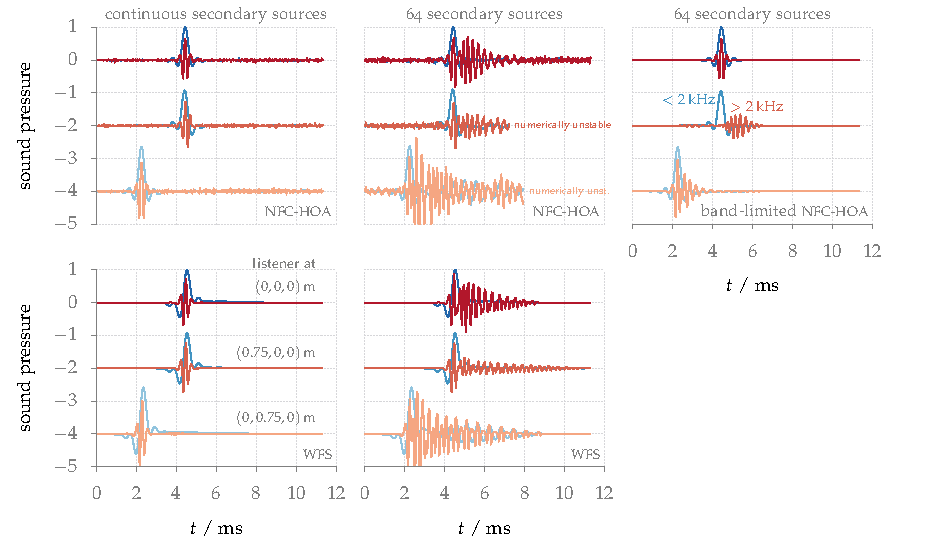
\includegraphics{fig3_15/fig3_15}
    \caption[][-3cm]{Sound pressure of a low and high-frequency cosine shaped
    impulse synthesized as plane wave by
    \ac{NFC-HOA}~\protect\eqref{eq:D_nfchoa_pw_25D} and
    \ac{WFS}~\protect\eqref{eq:d_wfs_pw_25D} at three listening positions. A
    fixed offset was added to the sound pressure at two listening positions for
    a better visualization. The low-frequency impulses are presented in blue, the
    high-frequency impulses in red.
    Parameters: $\xs = (0,-1,0)$, $\xref = (0,0,0)$\,m, circular secondary
    source distribution with a diameter of $3$\,m.
    \reproduce{\GITHUB/fig3_15}}
    \label{fig:sound_field_imp_fixed_filtered}
\end{figure*}
%
\newthought{An interesting question} is how different frequencies
are distributed in the unwanted wave fronts. Investigating this in
Figure\,\ref{fig:sound_field_imp_fixed_filtered}, a low frequency pulse with $f <
2$\,kHz and a high frequency pulse with $f > 2$\,kHz are synthesized. It is
evident that for the case of a continuous secondary source distribution,
both the low and the high frequencies are synthesized at the same time. For
the sampled secondary sources and the case of \ac{WFS} and \ac{NFC-HOA}, a common onset of
both pulses is visible, but the additional wave fronts contain only high
frequencies. The explanation is that frequencies below the
aliasing frequency are synthesized correctly, and errors in the synthesized
sound field are expected only for frequencies
above the aliasing frequencies.
In the case of band-limited \ac{NFC-HOA}, for the center position the low- and
high-frequency pulses arrive at the same time. On the other hand,
for both positions out of the
center the low and high frequencies disintegrate. At first only low
frequencies arrive at the listener's position, thereafter only high
frequencies.

\newthought{Focused sources} have similar aliasing properties as band-limited
\ac{NFC-HOA}. The difference is that the aliasing-free region is not around
the center of a circular secondary source distribution but around the
focused source position.
However, beside this they have some special properties that are obvious when
analyzing their time signal at a non aliasing free listener position. As
Figure\,\ref{fig:sound_field_imp_fixed_fs} indicates the additional
spatial aliasing wave fronts arrive before the desired one. This
is caused by the
time reversal approach\autocite{Yon2003} that is applied to produce the field
of a focused source and cannot be overcome -- compare~\eqref{eq:d_wfs_fs_25D}.
%
\begin{figure}[t]
    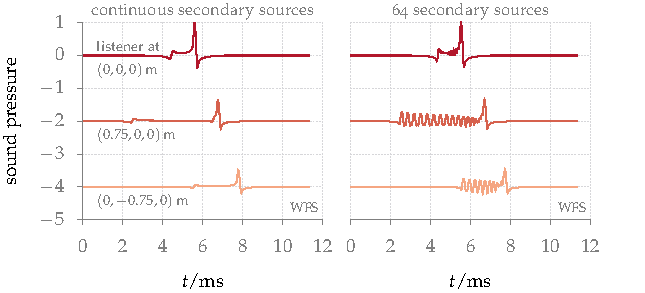
\includegraphics{fig3_16/fig3_16}
    \caption{Sound pressure of a cosine shaped impulse synthesized as focused
    source by \ac{WFS}~\protect\eqref{eq:d_wfs_fs_25D} at three listening
    positions. A fixed offset was added to the sound pressure at two listening
    positions for a better visualization.
    Parameters: $\xs = (0,0.5,0)$\,m, $\n_\text{s} = (0,-1,0)$, circular
    secondary source distribution with a diameter of $3$\,m.
    \reproduce{\GITHUB/fig3_16}}
    \label{fig:sound_field_imp_fixed_fs}
    \vspace{-0.7cm}
\end{figure}

\newthought{So far} this section has summarized the errors in the sound field due
to the spatial sampling process of the secondary sources. In the following paragraph
the possible influence of these errors on the perception of the sound field will be
discussed.


%----%----%----%----%----%----%----%----%----%----%----%----%----%----%----%----
\paragraph{Perception}
%
The discretization of the secondary source distribution may have a huge impact
on the perception of the synthesized sound field, as a result of the large amount
of errors which are introduced by the spatial sampling process.

Three perceptual features will strongly be influenced by the errors,
namely the localization of the synthesized sound, its perceived
timbre, and the perception of spectro-temporal artifacts.
These features will at first be discussed in the following and then analyzed
with dedicated experiments in Chapter\,\ref{cha:psychoacoustics}.

%
\begin{figure}[tb]
    \vspace{-0.5cm}
    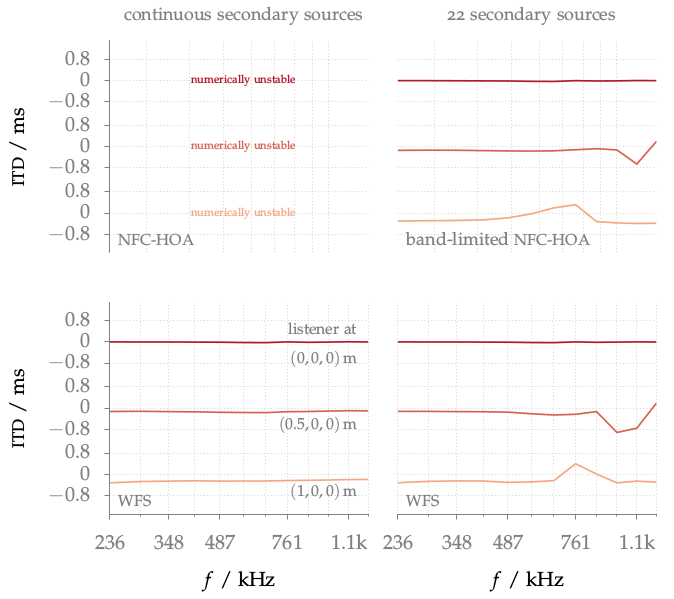
\includegraphics{fig3_17/fig3_17}
    \caption{\acp{ITD} for a pink noise signal synthesized as a point source by
    \ac{NFC-HOA}~\protect\eqref{eq:D_nfchoa_pw_25D} and
    \ac{WFS}~\protect\eqref{eq:d_wfs_pw_25D} at three listening
    positions, with a head orientation of $90\degree$.
    Parameters: $\xs =(0,2.5,0)$, $\xref = (0,0,0)$, circular secondary source
    distribution with a diameter of $3$\,m.
    \reproduce{\GITHUB/fig3_17}}
    \label{fig:sfs_itd}
\end{figure}
%
\newthought{For localization} it is worthwhile to analyze the influence of the
spatial aliasing on the \ac{ITD} of the sound field. It is especially
interesting for frequencies below $1.4$\,kHz, because for broad-band signals
localization in the horizontal plane
is dominated by the \acp{ITD} of low
frequencies.\sidenote[][-1cm]{\cite{Wightman1992}}
Figure\,\ref{fig:sfs_itd} shows the \ac{ITD} for synthesized signals of a
point source for three different listening positions with the head always
oriented to the front. The \acp{ITD} were
calculated applying the binaural model that is introduced in
Chapter\,\ref{cha:modelling}.
In case of a continuous secondary source distribution, the \acp{ITD} are correct, because
the sound field is not distinguishable from the desired one. For the sampled
secondary source distribution consisting of 22 sources in this analysis, deviations of the
\ac{ITD} above $500$\,Hz are visible. The $500$\,Hz roughly corresponds to
the aliasing frequency. By applying~\eqref{eq:fal} it can be calculated that a
distance of $12$\,cm between the secondary sources would be sufficient to
achieve correct \acp{ITD} below $1.4$\,kHz.

For \ac{WFS} and \ac{NFC-HOA} the first wave front which arrives at
the listener position is synthesized correctly. Subsequently, additional
wave fronts with disturbing directional information are arriving at the listener
position -- compare Figure\,\ref{fig:sound_field_imp_fixed_filtered}. The
additional wave fronts are carrying the directional information of the corresponding
secondary source they are coming from. This
case is comparable to the localization in closed spaces. There, after the
direct wave front additional reflectional wave fronts from the walls follow.
The localization is mostly dominated by the first wave front, a
phenomenon known as the precedence effect.\autocite[][]{Litovsky1999}
This leads to the hypothesis that localization for the case of \ac{SFS}
will be comparable to the case of a real sound field.
If the number of secondary sources is becoming so low that the first
wave front can no longer be synthesized correctly in the whole audience area,
impairments of localization are likely. This is the case for stereophony.

For band-limited \ac{NFC-HOA} this effect could also be critical for positions outside of the
center, because here the first wave front is only correct for low frequencies.
In contrast, wave fronts with high frequencies are coming from a different direction -- compare again
Figure\,\ref{fig:sound_field_imp_fixed_filtered}. In this situation
more than one source will probably be perceived.

Another case where the localization could be largely affected by the synthesis
errors is the synthesis of focused sources. Here the critical aspect is that the
correct wave front arrives after -- not before -- all the additional high
frequency wave fronts that arrive from false directions.

In Section\,\ref{sec:localization} the localization in case of different sound field
synthesis methods and for different synthesized sound sources like a point source
or a focused source is investigated in great detail. Afterwards, in
Chapter\,\ref{cha:modelling}, an auditory model is used to predict the
localization results and to predict the localization in the entire audience area.


\newthought{Coloration is} the other perceptual feature that is affected by
synthesis errors. Here, it is not as straightforward as for
the perception of the direction of the auditory event. There is
a correlation between the amount of perceived coloration and the
comb-filter like deviations in the magnitude of the
spectrum resulting from sound field synthesis -- compare
Figure\,\ref{fig:freq_response}. Similar deviations of the spectrum occur
also for stereophonic presentation and for auditory
perception in closed spaces, where room reflections could create a comb-filter
like spectrum. However, for stereophony, coloration plays only a minor
role.\autocite{Pulkki2001b} Further, in the case of closed spaces, not a colored
auditory event is perceived, but the coloration is perceived as separate
information about the acoustic properties of the room.
The perceived character of the space in terms of an independent
auditory event can then also be
perceived as colored. For example, the human listener seems to be
highly trained for natural patterns of reflections. Simulating a room
with a simple model including only the first reflections will sound
very unnatural, and different perceptual dimensions of coloration will be affected.

In the context of \ac{SFS} both deviations in the magnitude spectrum and
several reflection-like wave fronts will occur. Either of these might contribute
to the perceived coloration, which may correspond to an additional unnatural 
room impression. The amount of deviations and number of additional wave
fronts depend on the number and distance between the secondary sources. A
continuous secondary source distribution will not lead to coloration,
whereas a lower number might.
Section\,\ref{sec:timbral_fidelity} investigates these questions, and
the coloration of different \ac{WFS} systems will be compared to that of a two-channel
stereophony setup.

For cases without a spatio-temporally correct first wave front, the errors in the
synthesized sound field will also induce coloration, but it
is not straightforward to predict the degree of coloration. It depends on how many auditory events
the listener will perceive, and on the frequency content of the different
sources.


\newthought{Spectro-temporal artifacts} may become audible if a technical system
manipulates a given signal in an unnatural way, as it may happen for
audio codecs. These codecs can add artifacts to the original signal
that are, for example, perceivable as additional clicks.
Especially pre-echoes are very likely to become
perceivable as additional auditory events. Since the synthesized signal of a
focused source has additional wave fronts arriving as pre-echoes, it is likely
that these wave fronts are heard as independent auditory events -- compare
Figure\,\ref{fig:sound_field_imp_fixed_fs}.
In Section\,\ref{sec:spectro_temporal_artifacts}, this effect is investigated for
different secondary source setups and different listening positions.
Additionally, an approach is presented to avoid spectro-temporal artifacts
for the synthesis of focused sources.

\newthought{To investigate} the localization and coloration of synthesized
\linebreak {sources}, the
number of applied secondary sources has to be varied in a large range going
from only two or three up to a continuous secondary source distribution.
This could be as much as $7000$ sources for reaching an upper frequency of $20$\,kHz.
Beside the varying number of secondary sources, results for different listening positions
within the audience area are of interest: A similar impression of the
auditory scene in an extended audience area is one of the claimed benefits of
sound field synthesis.

It is obvious that these requirements represent a big challenge for the experimenter
because it is not possible to practically build secondary source distributions with up to
$7000$ sources and inter-loudspeaker distances of below $1$\,cm. Even the task of
positioning a listener reliably at different positions within the audience area
is not straightforward for practical evaluation tests.
To overcome these problems, all the
different secondary source distributions and listener positions are simulated
for this thesis
via dynamic binaural synthesis using headphones.

In the next section, the method of dynamic binaural synthesis is explained in
detail altogether with the experimental setups. Binaural synthesis is not
absolutely transparent and its limitations and restrictions are also
investigated and discussed.
